\section{Design}\label{s:design}
%
\begin{figure*}
    \centering
    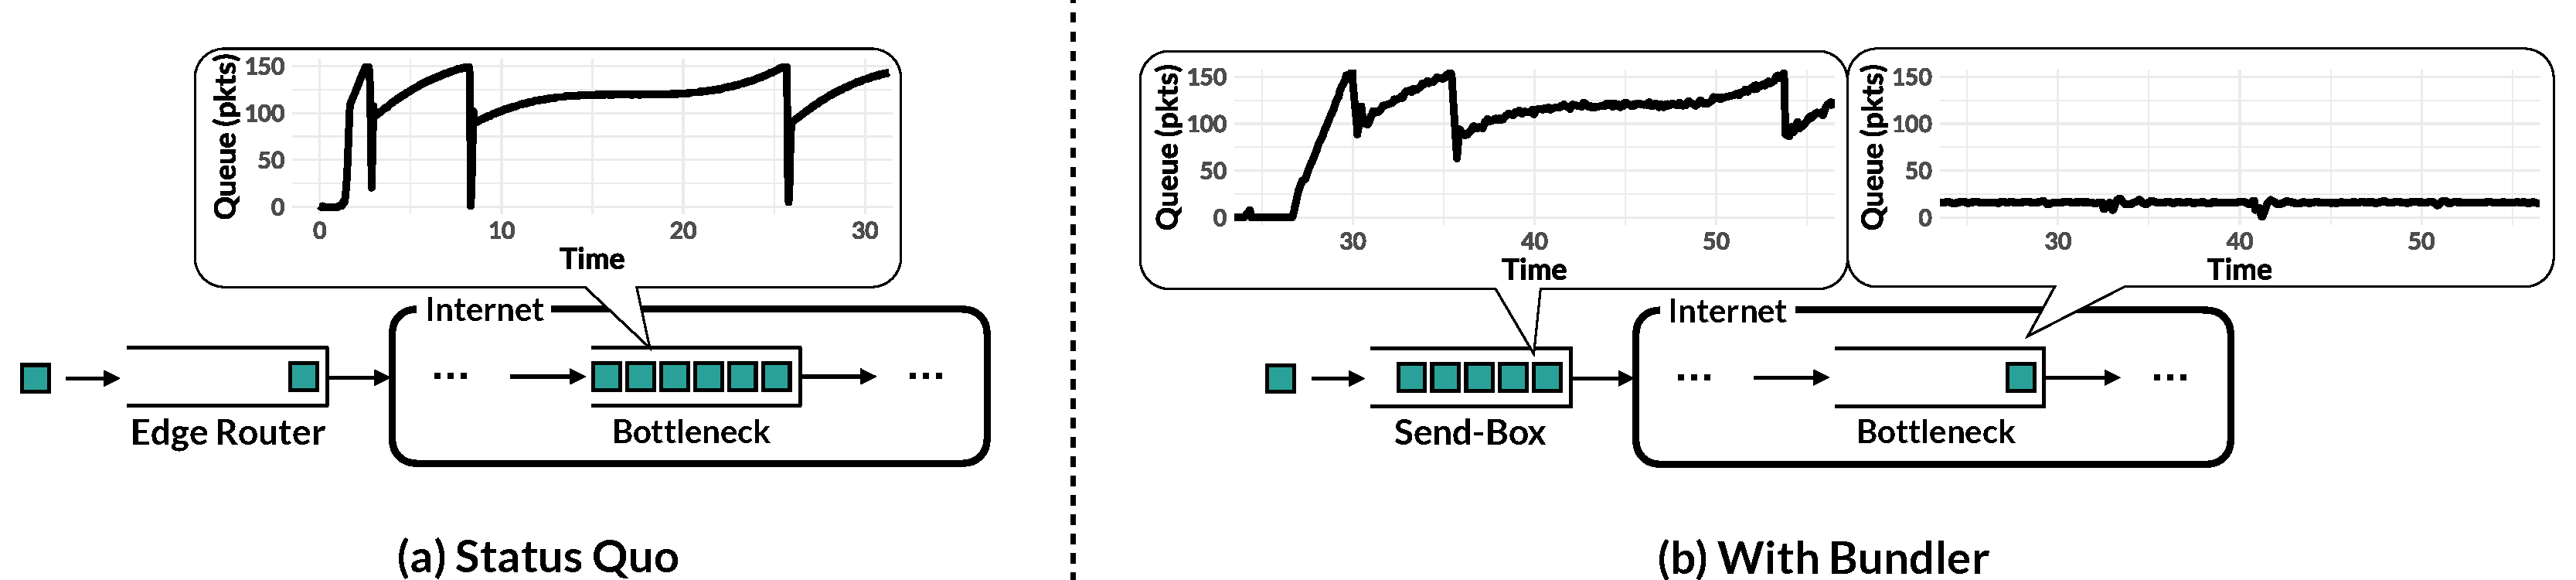
\includegraphics[width=\textwidth]{img/shift-bottleneck-combined}
    \caption{This illustrative example with a single flow shows how \name can take control of queues in the network. The plots show the trend in measured queueing delays at the relevant queue over time. The queue where delays build up can best make scheduling decisions, since it has the most choice between packets to send. Therefore, the \inbox \emph{shifts} the queues to itself to gain scheduling power.}\label{fig:design:shift-bottleneck}
\end{figure*}
%
\cut{
\an{maybe move to ``bundler's utility regime''/Overview/``Traffic Bundles'': 
What is the best way to take advantage of the existence of traffic bundles?
Broadly, there are two approaches: congestion control and in-network scheduling. 
Today, congestion control is a distributed concern: each end-host performs its own optimization to achieve the highest throughput and lowest latency.
Indeed, end-host rate control is a deployed method to enforce domain-wide scheduling policy in private WANs~\cite{bwe}.
On the other hand, scheduling is an in-network concern; existing proposals such as DiffServ~\cite{diffserv} observe that the network is uniquely positioned to differentiate between different flows according to some domain-wide policy.
Scheduling presents its own challenge: because the Internet is a federated system, the link with queue build-up (and thus with the opportunity to re-order packets according to a scheduling policy) will likely be outside the sending domain's purview.

\an{don't know what to say next}
}
}

Recall that in order to do scheduling, we need to move the queues from the network to the \name. 
In this section, we first describe our key insight for moving the in-network queues, and then explain our specific design choices. 
Our overriding design principle is simplicity; at various points in the design, there exists a more complex approach which we discard \an{rephrase}.
Recall that each domain deploys one \name middlebox which we logically partition into sender-side (\inbox) and receiver-side (\outbox) functionality.

\subsection{Key Insight}
One strategy for inducing queuing at the \inbox would be to set a low outgoing rate limit on outgoing traffic. 
However, if this rate is made smaller than the bundle's fair share of bandwidth at the bottleneck link in the network, it will decrease throughput. 
Conversely, if the rate is too high, packets will pass through the \inbox without queueing.
Instead, the rate needs to be set such that the bottleneck link sees a small queue while remaining fully utilized (and the bundled traffic competes fairly in the presence of cross traffic). 
We make a simple, but powerful, observation: existing congestion control algorithms calculate exactly this rate~\cite{Jacobson88}. 
Therefore, running such an algorithm to set a bundle's rate would reduce its self-inflicted queue at the bottleneck, causing packets to queue at the \inbox instead, without reducing the bundle's throughput.
Note that end hosts would continue running a traditional congestion control algorithm as before (\eg Cubic~\cite{cubic}, BBR~\cite{bbr}) which is unaware of \name.

Figure~\ref{fig:design:shift-bottleneck} illustrates this concept for a single flow traversing a bottleneck link in the network
\footnote{Details of the emulated network setup which resulted in the illustrated queue length time-series are in \S\ref{s:eval}.}.
Without \name, packets from the end hosts are queued in the network, while the queue at the edge is unoccupied. 
In contrast, a \name deployed at the edge is able to shift the queue to its \inbox.

\subsection{Design Overview}\label{s:design:overview}
\begin{figure}
    \centering
    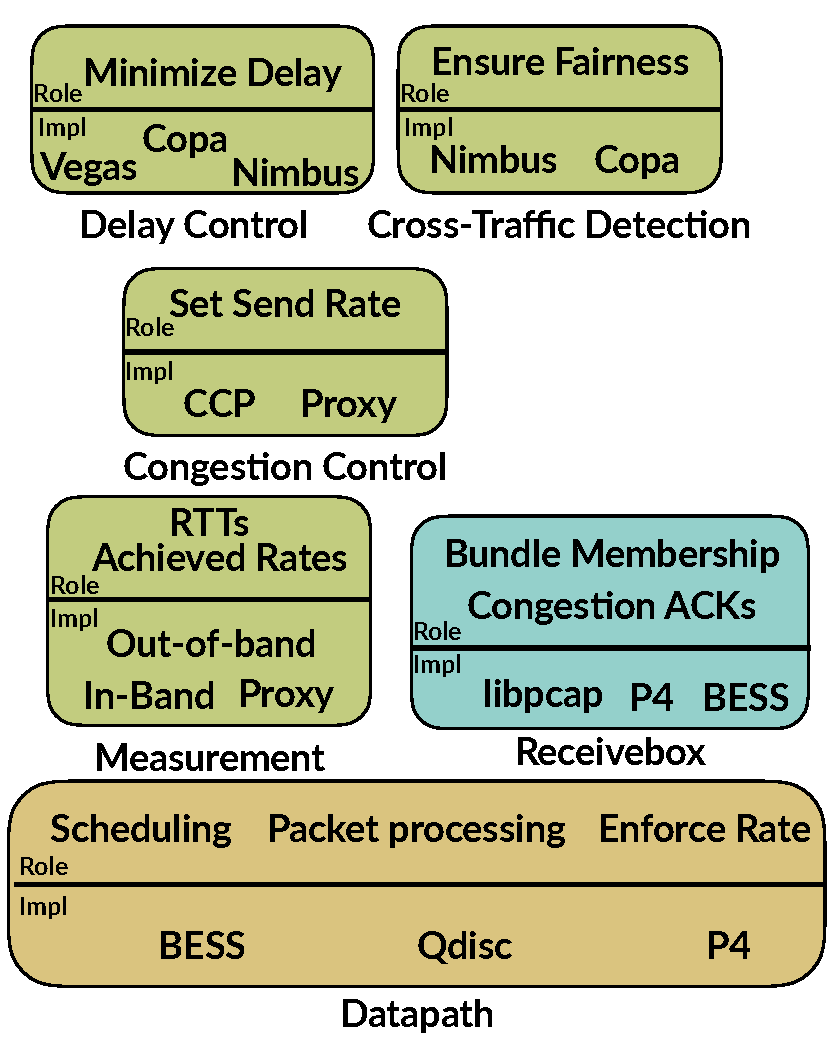
\includegraphics[width=\columnwidth]{img/arch-block-diag}
    \caption{\name comprises of five sub-systems: four (in green) implement \inbox functionality, one (in blue) implements \outbox functionality, and the datapath (orange) is shared between the two. \name's architecture supports multiple compatible implementations (listed in the ``Impl'' section of each block).}\label{fig:design:block-diag}
\end{figure}
Figure~\ref{fig:design:block-diag} shows the necessary components of any \name: (1) a means of determining bundle membership; (2) a rate enforcement mechanism; (3) a measurement strategy; (4) a delay-controller; and (5) a fairness-controller.
Throughout this section we discuss design options for determining Bundle membership (\S\ref{s:design:membership}), observing feedback (\S\ref{s:design:twosided}), and congestion control (\S\ref{s:design:whichcc}): for other aspects of the design, \name is compatible with a variety of options. For example, domains can implement \name using any modern middlebox datapath, \eg P4~\cite{p4}, BESS~\cite{bess}, or as in our prototype implementation (\S\ref{s:impl}), Linux tc qdiscs.

\an{maybe move congestion control choice before measurement?}

\subsection{Indentifying Bundle Membership}\label{s:design:membership}
\name must identify which packets (or flows) are part of the same traffic bundle.
It is important to only bundle those flows which share the same bottleneck; otherwise, \name may send a component flow at the wrong rate for its bottleneck.
This has traditionally been a difficult problem; multipath TCP~\cite{mptcp} sidesteps it with a weighted window increase-decrease protocol, 
and Rubenstein \etal~\cite{active-sharedbottlenecks} use a ``poisson-probing'' mechanism to probabilistically identify shared bottlenecks under a limited network model.

\an{better transition?}
We instead adopt a simple, direct, and more accurate approach: \emph{two-way opt-in}.
In this approach, a domain must agree to bundle traffic on both the sending and receiving sides.
The first step, of course, is to place a \name middlebox at the domain's edge.
Initially, the \inbox assumes all component traffic is unbundled.
When the \outbox observes an unbundled packet, it opts-in by sending a message \an{clarify not on every packet} containing the IP prefix it covers, addressed to the source IP of the packet
\footnote{Addressing to the source IP of the packet is not strictly necessary; domains may also advertise \inbox{}es via \eg DNS.}.
If there is no \inbox on the path, this message will be ignored.
Otherwise, a \inbox will observe this message and can opt-in by initializing a new traffic bundle corresponding to the \outbox's destination prefix.

%The \outbox does one of two things for each potential epoch boundary packet:
%\begin{enumerate}
%    \item If the packet is in a known bundle, the \outbox sends a message to the corresponding \inbox.
%    \item If the packet is not in a known bundle, the \outbox sends a message to the source IP address of that packet.
%\end{enumerate}

%The \inbox receives (and intercepts) the \outbox feedback.  
%The \inbox at this time updates its flow tables to add the destination IP of the epoch boundary packet either to an existing bundle (in the case of a new flow from a previously-unseen source subnet joining a bundle) or instantiates a new bundle.
%The \inbox then sends a response containing an epoch size to use and the hash of the epoch boundary packet.
%The \outbox receives this message, initializes a byte counter for the newly discovered bundle, and remembers the \inbox IP address for future feedback. If there is no \inbox on the path, the packet will simply be ignored at its destination. 

\subsection{Implementing Congestion Control}\label{s:design:twosided}
Congestion control algorithms we wish to run at the \inbox require network feedback from the receivers to measure congestion and adjust the sending rates accordingly. 

This problem presents multiple possible solutions:

\paragrapha{Passively observe in-band acknowledgements}
Conventional endhost-based implementations have used TCP acknowledgements to gather congestion control measurements.
However, this is not a good option for \name because 
it is specific to TCP and thus incompatible with alternate protocols, \ie UDP for video streaming or QUIC's encrypted transport header~\cite{quic}.

\paragrapha{Terminate connections and proxy through TCP} This approach allows the unmodified use of existing congestion control algorithms, since a TCP tunnel can collect ACKs. Furthermore, TCP proxies can improve performance by allowing end-to-end connections to ramp up their sending rates quickly.
The primary disadvantage of this approach is that \name must take responsibility for reliable delivery of component traffic, which requires large amounts of queueing and, in the case of UDP applications, can harm application performance. 
Furthermore, proxying TCP connections introduces a new potential point of failure at \name; if \name crashes, connections will be lost.
Finally, from a practical standpoint, to avoid head-of-line blocking this approach requires that \name open a new proxy connection for each component end-host connection, but still determine the bottleneck rate of the traffic \emph{aggregate}. While this approach may be technically feasible~\cite{cm}, the cycles used for opening and managing new proxy connections are better used for packet processing.
Thus, we set aside TCP tunnels for the remainder of this discussion, but note that this approach is complementary with \name (see \S\ref{s:eval}) \radhika{might need some rephrasing}.
\footnote{\an{If anyone still cares, from an architectural standpoint this design runs counter to the end-to-end principle~\cite{e2e-principle}; it replicates endhost functionality in the network.}}.
\radhika{we can now probably chop off the discussion of TCP proxy in related work?}

\an{discuss non-terminating tcp tunnels?}

\paragrapha{Out-of-band feedback} Having eliminated the options for using in-band feedback, we adopt out-of-band feedback in the form of congestion-specific ACKs: the \outbox sends out-of-band feedback to the \inbox.
This decouples congestion-specific ACKs from traditional ACKs used for reliability\footnote{The idea of a congestion ACK is similar to that in QCN~\cite{qcn}, although our goals differ.} and is thus indifferent to the underlying protocol (be it TCP, UDP, or QUIC).

\an{move to ``measuring congestion''?}
When should the \outbox send these feedback messages? 
Sending an out-of-band feedback message for every packet arriving at the \outbox would result in high communication overhead. 
Furthermore, conducting measurements on every outgoing packet at the \inbox would require maintaining state for each of them, which can be expensive, especially at high bandwidth-delay products. 
This overhead is unnecessary; reacting once per RTT is sufficient for congestion control algorithms~\cite{ccp}. 
We therefore sample a subset of the packets for which to receive congestion ACKs.

We detail the sampling mechanism and contents of congestion ACKs in \S\ref{s:measurement}.

\subsection{Choice of congestion control algorithm}\label{s:design:whichcc}
\name's congestion control algorithm must satisfy the following requirements: 

\paragraphi{(1) Ability to limit network queueing} \name must limit queueing in the network to move the queues to the \inbox. Therefore, congestion control algorithms which are designed to control delays, and thus queueing, are the appropriate choice. 
A window-probing congestion control algorithm which fills buffers (\eg Cubic, NewReno), for example, is not a good choice for \name, since it would build up a queue at the network bottleneck and drain queues at the \inbox.

\paragraphi{(2) Detection of buffer-filling cross-traffic} Simultaneously, it is well-known that delay-controlling schemes (\eg Vegas~\cite{vegas}) compete poorly with buffer-filling window-probing schemes~\cite{copa}.
Therefore, \name must have a mechanism to detect the presence of such competing buffer-filling flows and fall back to status quo performance, and then detect when they have left to take back its control over the network queues. 

The emergence of such detection mechanisms is recent: Copa~\cite{copa} detects whether it is able to empty the queues, and Nimbus\footnote{Concurrently submitted work: paper \an{XX} describes Nimbus.} provides a more general mechanism which overlays a pattern on the sending rate and measures the cross traffic's response.

Copa's detection mechanism does not work for \name, because it relies on emptying the queues; since a bundle may itself be comprised of buffer-filling traffic, the queues will not empty! Therefore, while Copa would be able to switch modes to compete with buffer-filling cross traffic, it would not be able to re-assert control over the queues once the cross traffic leaves.
Therefore, we use the more general Nimbus mechanism, which uses \emph{active probing} to differentiate between \name's own traffic and cross traffic in the bottleneck queue.

We discuss active probing in \S\ref{s:queue-ctl}.
